\documentclass[a4paper,11pt]{report}
\usepackage{Cours}
\usepackage[procnames]{listings}

\definecolor{keywords}{RGB}{250,50,000}
\definecolor{comments}{RGB}{0,130,000}
\definecolor{definitions}{RGB}{0,0,130}
\definecolor{red}{RGB}{160,0,0}
\definecolor{green}{RGB}{0,150,0}
\definecolor{lblue}{RGB}{173,216,230}
\definecolor{mygray}{rgb}{0.93,0.93,0.99}
\definecolor{mymauve}{rgb}{0.58,0,0.82}
\definecolor{colorstring}{rgb}{0.55,0.35,0.3}

\lstset{language=Python, 
		backgroundcolor=\color{mygray},	%Rajoute une couleur en fond
        basicstyle=\ttfamily\small, 			%Fonte et style de base
        keywordstyle=\color{keywords},		%Coloration des mots-cles
        morekeywords={False, True},			%On rajoute des mots-cles
		ndkeywordstyle=\color{mymauve},      %D'autres types de mots-cles de couleur différente
        ndkeywords={input, range, len, print, open},    %Les mots-cles en question  	
        commentstyle=\color{comments},		%Couleur des commentaires
        stringstyle=\color{colorstring},			%Couleur des chaines de caracteres
        showstringspaces=false,				%Visualisation des espaces dans les chaines
        breaklines=true,						%Permet le passage à la ligne (code wrap)
        numbers=left,                   		%Position de la numerotation des lignes
  		numbersep=8pt,                  	%La distance entre la numerotation des lignes et le code
  		numberstyle=\tiny\color{gray}, 	%Le style utilise pour la numerotation
  		rulecolor=\color{black},         	%A forcer sinon probleme de couleur lors des chgts de lignes avec du texte autre que noirs (commentaires par ex)
  		showspaces=false,                	%Visualise les espaces partout en rajoutant des _ partout. Ceci écrase 'showstringspaces'
  		showstringspaces=false,          	%Un _ n'est rajoute que pour les chaines
  		showtabs=false,                  	%Montre les tab dans les chaines ajoutant un _ particulier
  		stepnumber=1,                    	%Le pas entre chaque ligne numerotee, si c'est 1, elles le sont toutes.
  		tabsize=2,   		   				%Taille d'un tab
  		xleftmargin=2pt,  					%Marge gauche
        identifierstyle=\color{black},		%Couleur des identifiants
        procnamekeys={def,class},			%Ce qui définit les fonctions
        procnamestyle=\color{blue}\textbf,	%Couleur affectee aux fonctions et mise en gras
        %framexleftmargin=5mm, 
        %frame=shadowbox, 					%Type de cadre (effet d'ombre)
        rulesepcolor=\color{gray}}

\usepackage{tikz,tkz-tab}
\newcommand{\enc}[1]{\begin{center}\fbox{#1}\end{center}}
\newcommand{\mat}
{\end{array}\right )}
\newcommand{\Acc}
{
\left \{
\begin{array}}
\newcommand{\Mat}
{
\left (
\begin{array}}
\newcommand{\acC}
{\end{array}\right.}
\title{test}
\newcommand{\Sum}[2]{\ensuremath{\textstyle{\sum\limits_{#1}^{#2}}}}


\begin{document}

\begin{center}
\textit{{ {\huge Corrigé DM2}}}
\end{center}

\bigskip

\begin{center}
 \shadowbox{Partie 1}
\end{center}

\medskip


\begin{enumerate}
\item Soit $x \in \mathbb{R}$. Alors $f(x)$ existe si et seulement si $1+x>0$ et $x \neq 0$. Ainsi, 
\enc{$f$ est définie sur $\mathcal{D} = ]-1, 0[ \cup ]0 , + \infty[$}

\item On a :
$$ \boxed{ \ln(1+x) \underset{0}{=} x- \dfrac{x^2}{2} + o(x^2)}$$
donc 
$$ f(x)\underset{0}{=} 1 - \dfrac{x}{2} + o(x)$$
On en déduit que :
$$ \lim_{x \rightarrow 0} f(x) = 1$$
Ainsi,
\enc{$f$ est prolongeable par continuité en $0$ en posant $f(0)=1$}
\item Pour tout réel $x$ appartenant à $\mathcal{D}$, on a :
\begin{align*}
\dfrac{f(x)-f(0)}{x-0} & = \dfrac{f(x)-1}{x} \\
& \underset{0}{=} \dfrac{-x/2+o(x)}{x} \\
& \underset{0}{=} - \dfrac{1}{2} + o(1)
\end{align*}
On en déduit que :
$$ \lim_{x \rightarrow 0} \dfrac{f(x)-f(0)}{x-0} = - \dfrac{1}{2}$$
Ainsi,
\enc{$f$ est d\'erivable en $0$ et $f'(0)= - \dfrac{1}{2}$}
La fonction $f$ est dérivable sur $\mathcal{D}$ par quotient de deux fonctions qui le sont avec un dénominateur ne s'annulant pas sur $\mathcal{D}$. Pour tout $x \in \mathcal{D}$, on a :
\begin{align*}
f'(x) & = \dfrac{1/(x+1) \times x - \ln(x+1) \times 1}{x^2} \\
& = \dfrac{x/(x+1)- \ln(x+1)}{x^2} \\
& = \dfrac{x-(x+1)\ln(x+1)}{(x+1)x^2}
\end{align*}
En particulier :
\begin{align*}
f'(x)&  \underset{0}{=} \dfrac{x-(x+1)(x-x^2/2+o(x^2))}{(x+1)x^2} \\
&  \underset{0}{=}\dfrac{x-x^2-x+x^2/2+o(x^2)}{(x+1)x^2} \\
& \underset{0}{=}\dfrac{-x^2/2+o(x^2)}{(x+1)x^2} \\
& \underset{0}{=}\dfrac{-1/2+o(1)}{(x+1)} \\
\end{align*}
Ainsi,
$$ \lim_{x \rightarrow 0} f'(x) = - \dfrac{1}{2}= f'(0)$$
Ainsi, $f$ est dérivable sur $\mathcal{D}'$ (car dérivable sur $\mathcal{D}$ et en $0$) et $f'$ est continue sur $\mathcal{D}'$ (d'après les règles usuelles sur $\mathcal{D}$ et d'après la limite précédente en $0$). Finalement,
\enc{$f$ est de classe $C^{1}$ sur $\mathcal{D}^{\prime}$}

\item Pour tout $x \in \mathcal{D}$, on a :
$$ f'(x) = \dfrac{k(x)}{(x+1)x^2}$$
La fonction $k$ est dérivable sur $\mathcal{D}$ (par combinaison linéaire de fonctions qui le sont) et pour tout $x \in \mathcal{D}$, on a :
\begin{align*}
k'(x) & = 1 - 1 \times \ln(1+x)-(x+1) \times \dfrac{1}{1+x} \\
& = 1 - \ln(1+x) - 1 \\
& = - \ln(1+x)
\end{align*}
Ainsi, $k'(x)$ est positif si et seulement si $\ln(1+x)$ est négatif ou encore si et seulement si $x$ est négatif. Par quotient de limites, on a :
$$ \lim_{x \rightarrow -1^{-}} f(x)= + \infty$$
et en remarquant que 
$$ f(x) = \dfrac{\ln(1+x)}{1+x} \times \dfrac{1+x}{x} \underset{+ \infty}{\sim} \dfrac{\ln(1+x)}{1+x}$$
on a par théorème des croissances comparées :
$$ \lim_{x \rightarrow + \infty} f(x) = 0$$
On en déduit le tableau de variations suivant :

\begin{center}
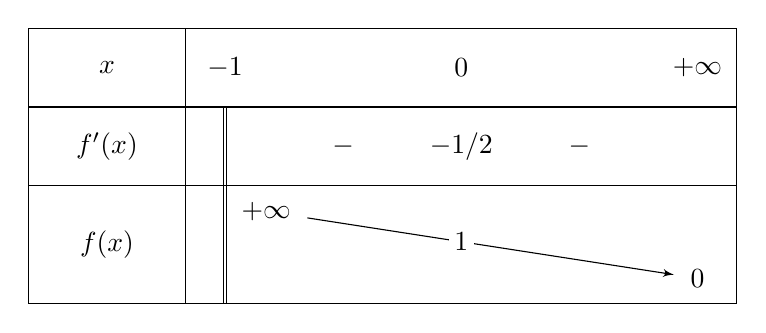
\begin{tikzpicture}
   \tkzTabInit{$x$ /1, $f'(x)$ /1, $f(x)$ /1.5} {$-1$ , $0$, $+ \infty$}
   \tkzTabLine{d, -, -1/2, -, } 
   \tkzTabVar{D+/ +$\infty$, R/, -/ 0}
   \tkzTabIma{1}{3}{2}{$1$}
\end{tikzpicture}
\end{center}
\end{enumerate}

\medskip

\begin{center}
 \shadowbox{Partie 2}
\end{center}

\medskip


\begin{enumerate}
\item La fonction $f$ est continue sur $[0,1]$ donc
\enc{$L$ est bien définie}

\item Soit $t \in [0,1]$. Par somme des termes d'une suite géométrique et sachant que $-t$ est différent de $1$, on a :
\begin{align*}
1-t+t^{2}-t^{3}+\cdots+\left(  -1\right)  ^{n-1}t^{n-1} & = \sum_{k=0}^{n-1} (-t)^k \\
& = \dfrac{1-(-t)^n}{1-(-t)}
\end{align*}
et ainsi,
$$ \boxed{1-t+t^{2}-t^{3}+\cdots+\left(  -1\right)  ^{n-1}t^{n-1}   =\dfrac{1-\left(  -1\right)
^{n}t^{n}}{1+t}}$$

\item Soit $x \in [0,1]$. L'égalité précédente est vraie pour tout $t \in [0,x]$ car $x \in [0,1]$ donc par intégration :
\begin{align*}
\int_0^x \dfrac{1-\left(  -1\right)^{n}t^{n}}{1+t} \dt & = \int_0^x 1-t+t^{2}-t^{3}+\cdots+\left(  -1\right)  ^{n-1}t^{n-1} \dt \\
& = \left[ t - \dfrac{t^2}{2} + \cdots + (-1)^{n-1} \dfrac{t^n}{n} \right]_0^x \\
& = x - \dfrac{x^2}{2} + \cdots + (-1)^{n-1} \dfrac{x^n}{n} \\
& = P_n(x)
\end{align*}
Par linéarité de l'intégrale, on a :
$$ \int_0^x \dfrac{1}{1+t} \dt - \int_0^x \dfrac{\left(  -1\right)^{n}t^{n}}{1+t} \dt = P_n(x)$$
ou encore 
$$ \left[\ln(1+t)\right]_0^x - \int_0^x \dfrac{\left(  -1\right)^{n}t^{n}}{1+t} \dt = P_n(x)$$
ce qui implique finalement que :
$$ \boxed{P_n(x) = \ln(1+x) - \int_0^x \dfrac{(-t)^{n}}{1+t} \dt }$$



\item Soient $n \geq 0$ et $x \in [0,1]$. D'après l'inégalité triangulaire (les bornes sont dans le bon sens), on a :
$$ \vert R_n(x) \vert \leq \int_0^x \left\vert \dfrac{(-t)^n}{1+t} \right\vert \dt  \leq \int_0^x \ \dfrac{t^n}{1+t} \dt$$
Or pour tout $t \in [0,x]$, $1+t \geq 1>0$ donc par décroissance de la fonction inverse sur $\mathbb{R}_+^{*}$:
$$ \dfrac{1}{1+t} \leq 1$$
et par positivité de $t^n$ :
$$ \dfrac{t^n}{1+t} \leq t^n$$
Par croissance de l'intégrale (les bornes sont dans le bon sens), on en déduit que :
$$  \vert R_n(x) \vert \leq \int_0^x \ \dfrac{t^n}{1+t} \dt \leq \int_0^x t^n \dt = \left[\dfrac{t^{n+1}}{n+1} \right]_0^x$$
et ainsi,

$$ \boxed{\left\vert R_{n}\left(  x\right)  \right\vert \leq
\dfrac{x^{n+1}}{n+1}}$$

\item Pour tout $x\in\left]  0,1\right]$,
$$ Q_{n}'\left(  x\right)  =1-\dfrac{x}{2}+\dfrac{x^{2}}{3}-\dfrac{x^{3}}{4}+\cdots+\left(  -1\right)^{n-1}\dfrac{x^{n-1}}{n}$$
et ainsi,
$$ \boxed{Q_{n}'\left(  x\right)=\dfrac{P_{n}\left(  x\right)  }{x}}$$


\item On sait que :
$$ \lim_{x \rightarrow 0} \dfrac{\ln\left(  1+x\right)  }{x}\ =1$$
et 
$$ \lim_{x \rightarrow 1} \dfrac{P_{n}\left(  x\right)  }{x}=1$$
On en déduit que $g_{n}\left(  x\right)$ tend vers $0$ (égal à $g_n(0)$) quand $x$ tend vers $0$ donc $g_n$ est continue en $0$ et donc sur $[0,1]$ par les règles usuelles. Il est donc licite de s'intéresser à l'intégrale de $\vert g_n\vert$ sur $[0,1]$.

\medskip

\noindent On sait que pour tout $x \in ]0,1]$,
$$Q_{n}'\left(  x\right)  =\dfrac{P_{n}\left(  x\right)  }{x}$$
Ainsi, en remarquant que $Q_n'(0)=1$, $Q_{n}$ est une primitive sur $[0,1]$ de 
$$x\rightarrow   \left\lbrace \begin{array}{cl}
\dfrac{P_{n}\left(  x\right)  }{x} & \hbox{ si } x \in ]0,1] \\[0.3cm]
1 & \hbox{ si } x=0 \\
\end{array}\right.$$
En remarquant que $Q_n'$ est continue sur $[0,1]$, on a :
\begin{align*}
\int_{0}^{1}g_{n}\left(  t\right)  \dt  & =\int_{0}^{1} Q_n'(t) \dt-\int_{0}^{1}f\left(  t\right)  \dt\\
& =\left[  Q_{n}\left(  t\right)  \right]  _{0}^{1}-L\\
& =Q_{n}\left(  1\right)  -Q_{n}\left(  0\right)  -L\\
& =Q_{n}\left(  1\right)  -L
\end{align*}
D'après l'inégalité triangulaire (les bornes sont dans le bon sens), on en déduit que :
\begin{align*}
\left\vert Q_{n}\left(  1\right)  -L\right\vert & =\left\vert \int_{0}^{1}g_{n}\left(  x\right)  \dx\right\vert\\
&  \leq\int_{0}^{1}\left\vert g_{n}\left(x\right)  \right\vert \dx
\end{align*}
Il reste \`a majorer $\left\vert g_{n}\left(  x\right)  \right\vert$ pour majorer ensuite l'int\'egrale de l'inégalité précédente. D'après la question 3, on a pour tout $x\in[0,1]$,
$$P_{n}\left(  x\right)  =\ln\left(  1+x\right)  -%
%TCIMACRO{\dint _{0}^{x}}%
%BeginExpansion
{\displaystyle\int_{0}^{x}}
%EndExpansion
\dfrac{\left(  -t\right)  ^{n}}{1+t}dt$$ 
donc
$$P_{n}\left(  x\right)  -\ln\left(  1+x\right)  =-%
%TCIMACRO{\dint _{0}^{x}}%
%BeginExpansion
{\displaystyle\int_{0}^{x}}
%EndExpansion
\dfrac{\left(  -t\right)  ^{n}}{1+t}dt$$
Ainsi, pour $x \neq 0$, 
$$\dfrac{P_{n}\left(  x\right)}{x}-\dfrac{\ln\left(  1+x\right)  }{x}=-\dfrac{1}{x}R_{n}\left(  x\right) $$
Ainsi, d'après la question $4$ et sachant que $x >0$,
\begin{align*}
\left\vert g_{n}\left(  x\right)  \right\vert &  =\left\vert \dfrac {P_{n}\left(  x\right)  -\ln\left(  1+x\right)  }{x}\right\vert \\
&  = \left\vert \dfrac{1}{x}R_{n}\left(  x\right)  \right\vert \\
& \leq\dfrac{1}{x}\dfrac{x^{n+1} }{n+1}\\
& =\dfrac{x^{n}}{n+1}
\end{align*} 
L'inégalité reste vraie pour $x=0$. Par croissance de l'intégrale (les bornes sont dans le bon sens), on en déduit que :
\[
\int_{0}^{1}\left\vert g_{n}\left(  x\right)  \right\vert dx\leq\int_{0}%
^{1}\dfrac{x^{n}}{n+1}dx=\dfrac{1}{\left(  n+1\right)  ^{2}}%
\]
Finalement, on a montré que :
\[
\boxed{0 \leq \left\vert Q_{n}\left(  1\right)  -L\right\vert \leq\int_{0}^{1}\left\vert
g_{n}\left(  x\right)  \right\vert dx\leq\dfrac{1}{\left(  n+1\right)  ^{2}}}
\]
On sait que :
$$ \lim_{n \rightarrow + \infty} \dfrac{1}{(n+1)^2} = 0$$
Par théorème d'encadrement, on en déduit que la suite de terme général $\vert Q_{n}\left(  1\right)  -L\vert$ converge vers $0$ et ainsi :
$$\boxed{\lim\limits_{n\rightarrow+\infty}Q_{n}\left(  1\right) = L}$$
\item Soit $N \geq 0$. $Q_{N}\left(  1\right) $ donne une valeur approch\'ee de $L$ \`a $10^{-4}$ près si :
$$\left\vert Q_{N}\left(  1\right)  -L\right\vert \leq10^{-4}$$
Il suffit que :
$$\dfrac{1}{\left(  N+1\right)  ^{2}}\leq10^{-4}$$
pour que l'inégalité précédente soit vérifiée. Raisonnons par équivalences :
\begin{align*}
\dfrac{1}{\left(  N+1\right)  ^{2}}\leq10^{-4} & \Longleftrightarrow 10^4 \leq (N+1)^2 \\
& \Longleftrightarrow 10^2 \leq N+1 \hbox{ (termes positifs)} \\
& \Longleftrightarrow 99 \leq N
\end{align*}
Ainsi,
\enc{La valeur approch\'ee est obtenue pour $N=99$}
\item Voici une proposition de solution :
\begin{lstlisting}
def Appr(eps):
    N=1
    S=1 # Valeur de QN(1)
    while 1/((N+1)**2) >eps:
        N=N+1
        S=S+(-1)**(N-1)/(N**2)
    return S
\end{lstlisting}
\end{enumerate}

\medskip

\begin{center}
 \shadowbox{Partie 3}
\end{center}

\medskip

\begin{enumerate}
\item La fonction $f$ est le quotient de deux fonctions de classe $\mathcal{C}^{\infty}$ sur $]0, + \infty[$ avec un dénominateur ne s'annulant pas donc 

\enc{$f$ est ind\'efiniment d\'erivable $\left]  0,+\infty\right[$}

\item On sait que pour tout réel $x>0$,

$$f^{\prime}\left(  x\right)  =\dfrac{x-\left(  1+x\right)  \ln\left(
1+x\right)  }{x^{2}\left(  1+x\right)  }=\dfrac{k\left(  x\right)  }%
{x^{2}\left(  1+x\right)  }$$
%
%Solution: $-\dfrac{1}{x^{2}}\dfrac{x-\left(
%\ln\left(  x+1\right)  \right)  \left(  x+1\right)  }{\left(  x+1\right)
%^{2}}-\dfrac{2}{x^{3}}\dfrac{x-\left(  \ln\left(  x+1\right)  \right)  \left(
%x+1\right)  }{x+1}-\allowbreak\dfrac{1}{x^{2}}\dfrac{\ln\left(  x+1\right)
%}{x+1}$ donc (on regroupe les termes en $\ln\left(  1+x\right)  $ pour
%r\'epondre \`a la question suivante)
On en déduit que pour tout réel $x>0$,
\begin{align*}
f^{\prime\prime}\left(  x\right)   & =\dfrac{k^{\prime}\left(  x\right)
x^{2}\left(  1+x\right)  -k\left(  x\right)  \left[  2x\left(  1+x\right)
+x^{2}\right]  }{x^{4}\left(  1+x\right)  ^{2}}\\\
& =x\dfrac{-\ln\left(  1+x\right)  x\left(  1+x\right)  -\left[  x-\left(
1+x\right)  \ln\left(  1+x\right)  \right]  \left[  2\left(  1+x\right)
+x\right]  }{x^{4}\left(  1+x\right)  ^{2}}\\
& =\dfrac{-x\ln\left(  1+x\right)  \left(  1+x\right)  -\left[  x-\left(
1+x\right)  \ln\left(  1+x\right)  \right]  \left[  2+3x\right]  }%
{x^{3}\left(  1+x\right)  ^{2}}\\
& =\dfrac{\left(  -x+2+3x\right)  \ln\left(  1+x\right)  \left(  1+x\right)
-x\left(  2+3x\right)  }{x^{3}\left(  1+x\right)  ^{2}}\\
& =\dfrac{\left(  2+2x\right)  \ln\left(  1+x\right)  }{x^{3}\left(
1+x\right)  }-\dfrac{2+3x}{x^{2}\left(  1+x\right)  ^{2}}\\
& = \boxed{2\dfrac{\ln\left(  1+x\right)  }{x^{3} }-\dfrac
{2+3x}{x^{2}\left(  1+x\right)  ^{2}}}
\end{align*}

\item Posons pour tout entier $n \geq 0$,

\begin{center}
$\mathcal{P}(n)$ : \og $\exists \, T_n \in \mathbb{R}[X], \exists a_n \in \mathbb{R} \, \vert \, \forall x>0, \; f^{\left(  n\right)  }\left(
x\right)  =\dfrac{T_{n}\left(  x\right)  }{\left(  1+x\right)  ^{n}x^{n}%
}+a_{n}\dfrac{\ln\left(  1+x\right)  }{x^{n+1}}$ \fg
\end{center}

\begin{itemize}
\item \textit{Initialisation.} On sait que pour tout réel $x>0$,
$$ f'(x) = \dfrac{x-\left(  1+x\right)  \ln\left(
1+x\right)  }{x^{2}\left(  1+x\right)  } = \dfrac{1}{x\left(  1+x\right)  } - \dfrac{ \ln\left(
1+x\right)  }{x^{2}}$$
En posant $T_1=1$ et $a_1=-1$, l'initialisation est donc vérifiée.
\item \textit{Hérédité.} Soit $n \in \mathbb{N}$ tel que $\mathcal{P}(n)$ soit vraie : 
$$ \exists \, T_n \in \mathbb{R}[X], \exists a_n \in \mathbb{R} \, \vert \, \forall x>0, \; f^{\left(  n\right)  }\left(
x\right)  =\dfrac{T_{n}\left(  x\right)  }{\left(  1+x\right)  ^{n}x^{n}%
}+a_{n}\dfrac{\ln\left(  1+x\right)  }{x^{n+1}} = \dfrac{T_{n}\left(  x\right)  }{(\left(  1+x\right) x) ^{n}%
}+a_{n}\dfrac{\ln\left(  1+x\right)  }{x^{n+1}}$$
On a alors pour tout réel $x>0$ :
\begin{align*}
f^{\left(  n+1\right)  }\left(  x\right)   & =\dfrac{T_{n}'\left(
x\right)  }{\left(  1+x\right)  ^{n}x^{n}}+T_{n}(x)\dfrac{-n(1+2x)}{\left(  1+x\right)
^{n+1}x^{n+1}}+a_{n}\dfrac{1}{1+x}\dfrac{1}{x^{n+1}}-\left(  n+1\right)
a_{n}\dfrac{\ln\left(  1+x\right)  }{x^{n+2}}\\
& =\dfrac{x\left(  1+x\right)  T_{n}'\left(  x\right)  -n\left(
1+2x\right)  T_{n}(x)+a_{n}\left(  1+x\right)  ^{n}}{\left(  1+x\right)
^{n+1}x^{n+1}}-\left(  n+1\right)  a_{n}\dfrac{\ln\left(  1+x\right)
}{x^{n+2}}%
\end{align*}
Posons :
$$ T_{n+1} =X\left(  1+X\right)  T_{n}'  -n\left(  1+2X\right)  T_{n}+a_{n}\left(  1+X\right)  ^{n}$$
\end{itemize}
$T_n$ est un polynôme à coefficients réels donc $T_{n+1}$ aussi. En posant $a_{n+1}= -(n+1)a_n$, on a alors :
$$ \forall x>0, \; f^{\left(  n+1\right)  }\left(
x\right)  =\dfrac{T_{n+1}\left(  x\right)  }{\left(  1+x\right)  ^{n+1}x^{n+1}%
}+a_{n+1}\dfrac{\ln\left(  1+x\right)  }{x^{n+2}}$$
L'hérédité est donc vérifiée. Ainsi, la propriété est vérifiée au rang $1$ et est héréditaire donc par principe de récurrence, elle est vraie pour tout entier $n \geq 1$.

\medskip

\noindent Finalement, pour tout entier naturel $n$ non nul il existe un polyn\^ome
$T_{n}$ \`a coefficients r\'eels et un r\'eel $a_{n}$ tels que :%
\[
\boxed{\forall x\in\mathbb{R}_{+}^{*},\quad f^{\left(  n\right)  }\left(
x\right)  =\dfrac{T_{n}\left(  x\right)  }{\left(  1+x\right)  ^{n}x^{n}%
}+a_{n}\dfrac{\ln\left(  1+x\right)  }{x^{n+1}}}
\]


\item Montrer par récurrence que pour tout entier $n \geq 1$, les coefficients de $T_{n}$ sont des entiers.

\begin{itemize}
\item \textit{Initialisation.} On sait que $T_1=1$ donc la propriété est vérifiée au rang $1$.
\item \textit{Hérédité.} Soit $n \geq 1$ tel que $T_{n}$ soit \`a coefficients entiers. Alors  $T_{n}',$ et $\left(  1+X\right)  ^{n}$ sont aussi à coefficients entiers et d'après la question précédente,
$$T_{n+1}  =X\left(  1+X\right)  T_{n}'\  -n\left(  1+2X\right)  T_{n}+a_{n}\left(  1+X\right)  ^{n}$$
est aussi un polynôme à coefficients entiers.  La propriété est donc vérifiée au rang $1$ et est héréditaire donc par principe de récurrence, elle est vraie pour tout entier $n \geq 1$.
\end{itemize}
Ainsi, 
\enc{pour tout entier $n \geq 1$, les coefficients de $T_{n}$ sont des entiers}
\item Pour utiliser la formule de Leibniz, on remarque que $f= g \times h$ où pour tout réel $x>0$,
$$g\left(
x\right)  =\dfrac{1}{x} \; \hbox{ et } \; h\left(  x\right)  =\ln\left(  1+x\right)  $$
On montre par récurrence (après conjecture) que pour tout entier $n \geq 0$ et tout réel $x>0$,
$$ g^{\left(  n\right)  }\left(  x\right)  =\dfrac{n!\left(
-1\right)  ^{n}}{x^{n+1}} $$
et de même pour tout entier $n \geq 1$ et tout réel $x>0$,
$$ h^{\left(  n\right)
}\left(  x\right)  =\dfrac{\left(  n-1\right)  !\left(  -1\right)  ^{n-1}%
}{\left(  1+x\right)  ^{n}}$$ 
D'après la formule de Leibniz, on a pour tout entier $n \geq 0$,
\begin{align*}
f^{\left(  n\right)  }\left(  x\right)   & =\sum_{k=0}^{n}\binom{n}%
{k}h^{\left(  k\right)  }\left(  x\right)  g^{\left(  n-k\right)  }\left(
x\right) \\
& =\binom{n}{n}\ln\left(  1+x\right)  \dfrac{\left(  -1\right)  ^{n}n!}{x^{n+1}%
}+\sum_{k=1}^{n}\binom{n}{k}\dfrac{\left(  k-1\right)  !\left(  -1\right)
^{k-1}}{\left(  1+x\right)  ^{k}}\dfrac{\left(  n-k\right)  !\left(
-1\right)  ^{n-k}}{x^{n-k+1}}%
\end{align*}
En utilisant l'expression de $\dis \binom{n}{k}$ avec les factorielles et en sortant les constantes de la somme, on a :
\begin{align*}
 \sum_{k=1}^{n}\binom{n}{k}\dfrac{\left(  k-1\right)  !\left(  -1\right)
^{k-1}}{\left(  1+x\right)  ^{k}}\dfrac{\left(  n-k\right)  !\left(
-1\right)  ^{n-k}}{x^{n-k+1}}&  =\sum_{k=1}^{n}\left(  -1\right)  ^{n-1}\dfrac{n!\left(
k-1\right)  !\left(  n-k\right)  !}{k!\left(  n-k\right)  !}\dfrac{\left(
1+x\right)  ^{n-k}x^{k-1}}{\left(  1+x\right)  ^{n}x^{n}}\\
& =\dfrac{1}{\left(  1+x\right)  ^{n}x^{n}}\left(  -1\right)  ^{n-1}%
n!\sum_{k=1}^{n}\dfrac{1}{k}\left(  1+x\right)  ^{n-k}x^{k-1}%
\end{align*}
On sait aussi que pour tout $x>0$, 
$$ f^{\left(  n\right)  }\left(
x\right)  =\dfrac{T_{n}\left(  x\right)  }{\left(  1+x\right)  ^{n}x^{n}%
}+a_{n}\dfrac{\ln\left(  1+x\right)  }{x^{n+1}}$$
Sachant que $a_1=-1$ et pour tout entier $n \geq 1$, $a_{n+1}=-(n+1)a_n$. Par une récurrence immédiate, on montre que pour tout entier $n \geq 1$,
$$ a_n = (-1)^n n!$$
Ainsi, pour tout $x>0$,
$$ f^{\left(  n\right)  }\left(
x\right)  =\dfrac{T_{n}\left(  x\right)  }{\left(  1+x\right)  ^{n}x^{n}%
}+\dfrac{(-1)^n n!\ln\left(  1+x\right)  }{x^{n+1}}$$
et 
\begin{align*}
f^{\left(  n\right)  }\left(  x\right)   & =\binom{n}{n}\ln\left(  1+x\right)  \dfrac{\left(  -1\right)  ^{n}n!}{x^{n+1}%
}+\dfrac{1}{\left(  1+x\right)  ^{n}x^{n}}\left(  -1\right)  ^{n-1}%
n!\sum_{k=1}^{n}\dfrac{1}{k}\left(  1+x\right)  ^{n-k}x^{k-1} \\
&  =\ln\left(  1+x\right)  \dfrac{\left(  -1\right)  ^{n}n!}{x^{n+1}%
}+\dfrac{1}{\left(  1+x\right)  ^{n}x^{n}}\left(  -1\right)  ^{n-1}%
n!\sum_{k=1}^{n}\dfrac{1}{k}\left(  1+x\right)  ^{n-k}x^{k-1} 
\end{align*}
On en déduit que pour tout $x>0$,
$$ \dfrac{T_{n}\left(  x\right)  }{\left(  1+x\right)  ^{n}x^{n}%
} = \dfrac{1}{\left(  1+x\right)  ^{n}x^{n}}\left(  -1\right)  ^{n-1}%
n!\sum_{k=1}^{n}\dfrac{1}{k}\left(  1+x\right)  ^{n-k}x^{k-1} $$
Ainsi,
$$\boxed{T_{n}  =\left(  -1\right)  ^{n-1}n!\sum
_{k=1}^{n}\dfrac{1}{k}\left(  1+X\right)  ^{n-k}X^{k-1}}$$
Pour $n=2$, d'après la question $2$, on sait que :
$$T_{2}\left(  X\right)  =-2-3X$$
et on a :
$$ \left(  -1\right)  ^{2-1}2!\sum_{k=1}^{2}\dfrac{1}{k}\left(  1+X\right)  ^{2-k}X^{k-1}=-2\left(  \left(  1+X\right)  ^{1}%
+\dfrac{1}{2}X\right)  =-2-3X$$ 
ce qui redonne bien l'égalité. 
\end{enumerate}




\end{document}